\documentclass[12pt, handout=show,notes=show]{beamer}

\usetheme[width=2cm]{Singapore}
\usecolortheme{rose}


%%%%lualatex on
%\usepackage{luatextra}
%\usepackage{fontspec}
\usepackage{amsmath}
%Ligatures={Contextual, Common, Historical, Rare, Discretionary}
%\setmainfont[Mapping=tex-text]{Linux Libertine O}

\usepackage{natbib}
\usepackage{mathptmx}
\usepackage{latexsym}
\usepackage{mathtools}
\usepackage[utf8x]{inputenc}
\usepackage[T1]{fontenc}


\DeclarePairedDelimiter\abs{\lvert}{\rvert}%
\DeclarePairedDelimiter\norm{\lVert}{\rVert}%


\makeatletter
\let\oldabs\abs
\def\abs{\@ifstar{\oldabs}{\oldabs*}}
\let\oldnorm\norm
\def\norm{\@ifstar{\oldnorm}{\oldnorm*}}
\makeatother

\title{\emph{Ceci n'est pas de l'arch\'eologie?}\\
	A Bayesian approach to understand consumption dynamics in Ancient Rome\\
}

\date{\tiny The Student Conference on Complexity Science (SCCS)\\
9th ­11th september 2015\\
Granada}
\author{\footnotesize Mar\'ia Coto-Sarmiento (Barcelona Supercomputing Center)\\
Xavier Rubio-Campillo (Barcelona Supercomputing Center)\\
José Remesal (University of Barcelona)}
\institute[]{

	EPNet Project \\
    Production and distribution of food during the Roman Empire:\\
    Economic and political dynamics

}


\begin{document}
\begin{frame}
  \maketitle
\vspace{-.8cm}
\begin{center}
		
\includegraphics[height=0.095\textwidth]{./epnetlogo.jpg}
		\hfil 
\includegraphics[height=0.080\textwidth]{./computing.jpg}
		\hfil 
\includegraphics[height=0.090\textwidth]{./ERC.png}

\end{center}
\end{frame} 


\section{Outline}

\begin{frame}{Outline}

\vfil
\begin{itemize}
\item Introduction
\item Quantitative Analysis: Bayesian Method
\item Archaeological data
\item Methods and Results
\item Discussion 
\item Conclusion

\end{itemize}

\end{frame}

\begin{frame}{Historical context}

\vfil
\begin{itemize}
\item Roman Empire is considered as one of main economic networks of the Mediterranean trade
\item The archaeological records allow to show the complex dynamics of consumption
\item Consumption dynamics can be detected for the distribution of the pottery

\end{itemize}

\begin{center}
		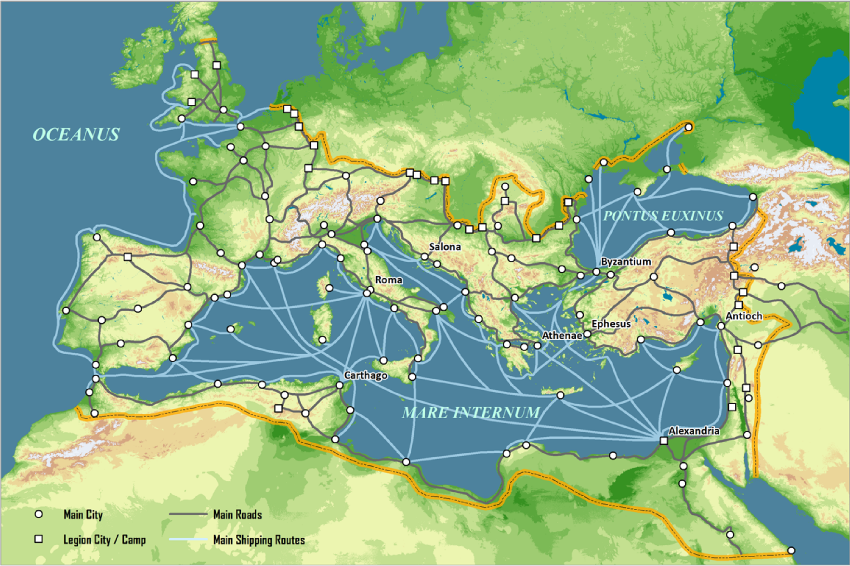
\includegraphics[height=0.23\textwidth]{./romanempire.png}
	   \hfil 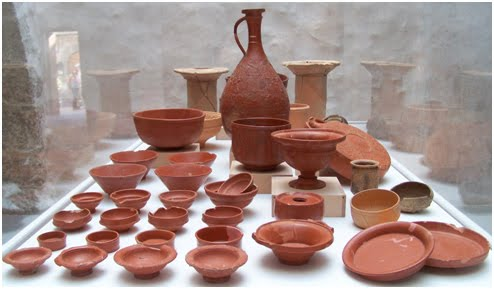
\includegraphics[height=0.23\textwidth]{./vajilla.jpg}
		
\end{center}

\end{frame}

\begin{frame}{Research Questions}
\begin{itemize}
\item
\Large Was the Roman economy a free market?\\
\item
\Large What was under the control of the Roman Empire? 
\end{itemize}

\end{frame}


\begin{frame}{Main challenges}

What are we going to find?\\
\vspace{0.5cm}
\begin{itemize}
\item "Inaccurate" historical sources to develop a hypothesis 
\item Poor quality of archaeological data
\item High levels of uncertainty associated to the archaeological dataset
\end{itemize}

\end{frame}

\section{Data}

\begin{frame}{Case Study}
\begin{itemize}

\item Monte Testaccio (Rome, Italy)
\item Artificial mount composed of fragments of broken amphorae 
\item Amphorae from Baetica (mostly), Africa and Gaul	
\item 1st-3rd centuries AD

\end{itemize}

\begin{center}
		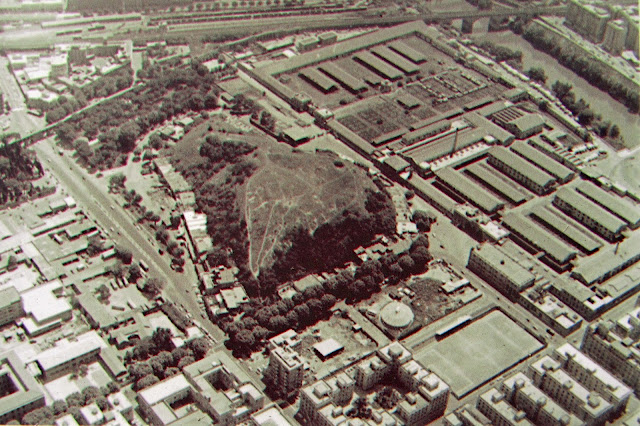
\includegraphics[height=0.3\textwidth]{./Mount-Testaccio2.jpg}
		\hfil 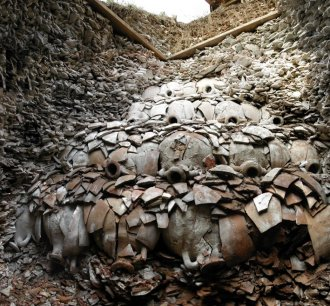
\includegraphics[height=0.3\textwidth]{./Mount-Testaccio.jpg}\\
		\vfill
	
\end{center}		

\end{frame}

\begin{frame}{Case Study: Archaeological data}
Dressel 20\\
\begin{itemize}
\item Amphorae stamps
\item \emph{Tituli picti}
\end{itemize}

\begin{center}
		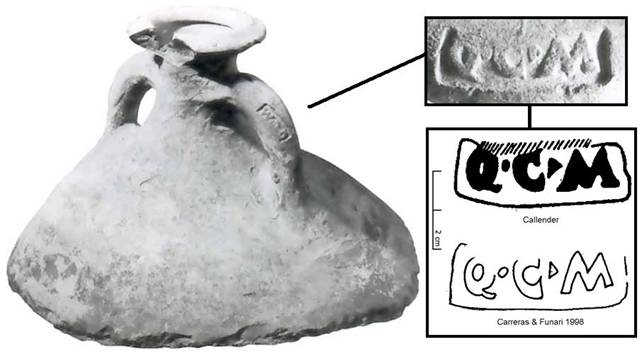
\includegraphics[height=0.3\textwidth]{./amphorae1.jpg}
		\hfil 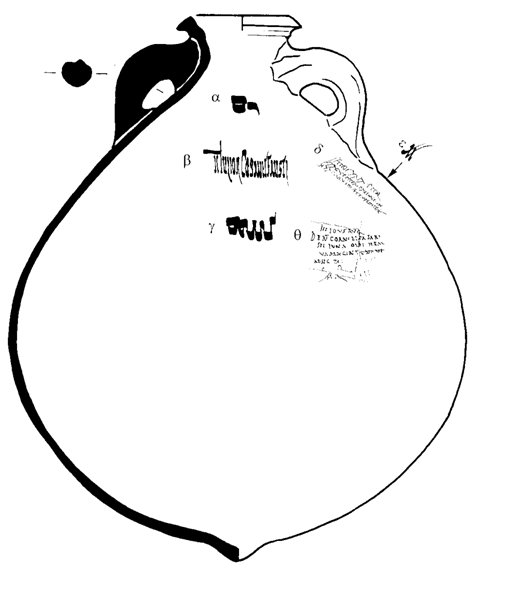
\includegraphics[height=0.3\textwidth]{./amphora.jpg}\\
		\vfill
	
\end{center}		

\end{frame}

\section{Method}

\begin{frame}{Approach}
\begin{itemize}
\item Analyse the economic activities from data of \emph{Monte Testaccio}
\item Ideal data:
\begin{itemize}
\item Analysis of frequency of distribution of different producers (type Dressel 20)
\end{itemize}
\item Proxy data
\begin{itemize}
\item Stamps are used as proxy-data to measure this frequency   
\end{itemize}
\end{itemize}
\end{frame}


\begin{frame}{A Method to analyse}
\begin{itemize}
\item Define a statistical model to each hypothesis
\item Explore the codes found in the stamps (different producers) 
\item We measure the frequency distribution of each one   
\end{itemize}

\begin{center}
		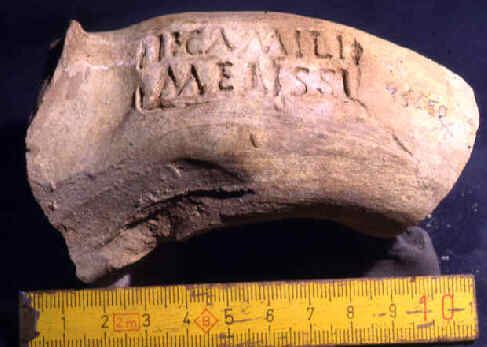
\includegraphics[height=0.3\textwidth]{./melissistamp.jpg}
		\hfil 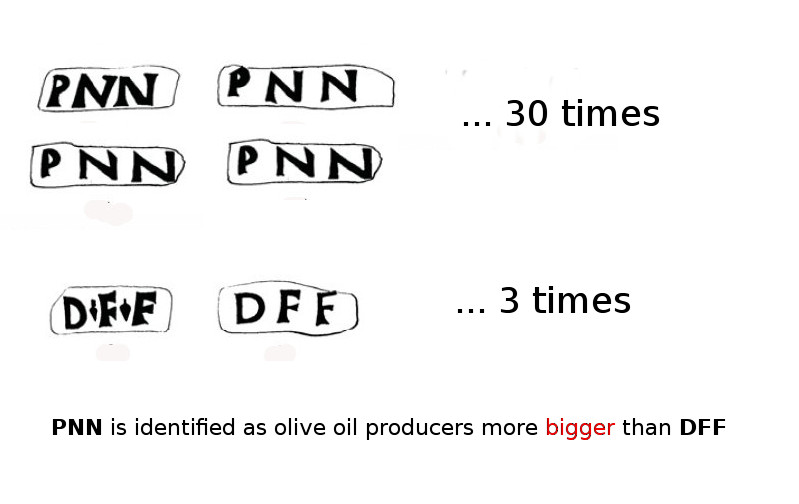
\includegraphics[height=0.3\textwidth]{./stamps.jpg}\\
		\vfil
	
\end{center}		
\end{frame}

\begin{frame}{Hypotheses}
\begin{itemize}
\item 1. The demand of olive oil was covered by small-size agents (producers)
\item 2. Presence of major producers (State control)
\item 3. Small-size producers survive to the increase and concentration of lands in hands of few producers
\item 4. Pareto principle: 80/20. 
\end{itemize}
\end{frame}

\section{Quantitative Analysis}

\begin{frame}{Quantitative analysis of archaeological data}
 Why \textbf{Bayesian Method} in Archaeology...?\\
 \vspace{0.5cm}
\begin{itemize}
\item Quantitative methods provide a scientist basis to the archaeological data
\item Possibility of testing what model explains better the evidence 
\item Integrates the level of uncertainty in archaeology
\end{itemize}

\end{frame}


\begin{frame}{M1: Poisson distribution}
\begin{itemize}
\item The demand of olive oil was covered by small agents (producers)
\item Frequency of producers
\end{itemize}
\begin{center}
		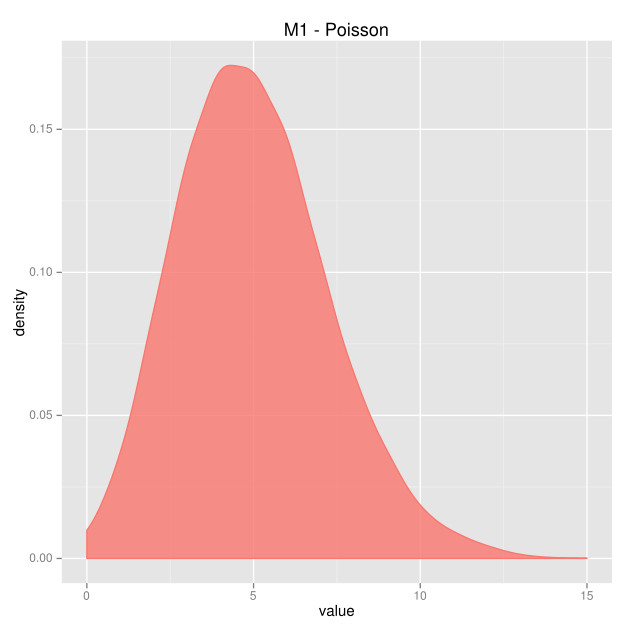
\includegraphics[height=0.5\textwidth]{./poisson.jpg}
		\vfill
\end{center}	
\begin{center}
\tiny Parameter: Lambda (U(1,30))
\end{center}

\end{frame}

\begin{frame}{M2: Negative binomial}
\begin{itemize}
\item Add variance: presence of major producers (State Control)
\end{itemize}
\begin{center}
		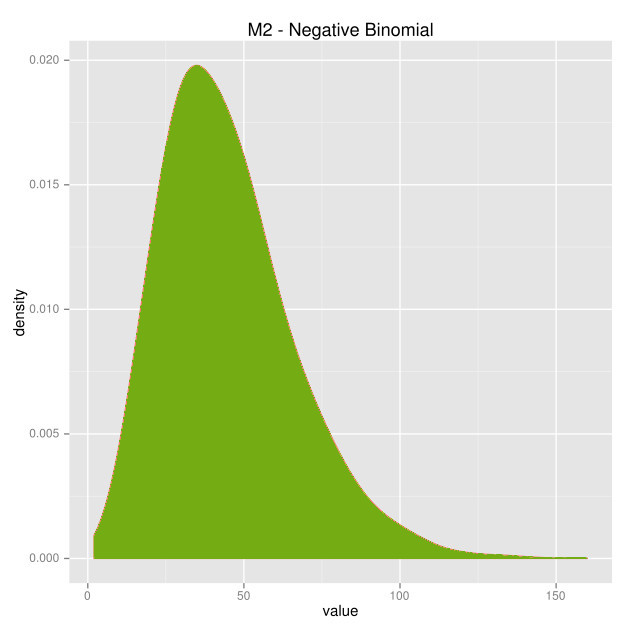
\includegraphics[height=0.5\textwidth]{./negative.jpg}
		\vfill
	
\end{center}	
\begin{center}
\tiny Parameters: size (U(1,100)) prob (U(0,1))
\end{center}

\end{frame}

\begin{frame}{M3: Lognormal distribution}
\begin{itemize}
\item Small producers survive to the increase and concentration of lands in hands of few producers
\item Concentration of land in few hands 
\end{itemize}
\begin{center}
		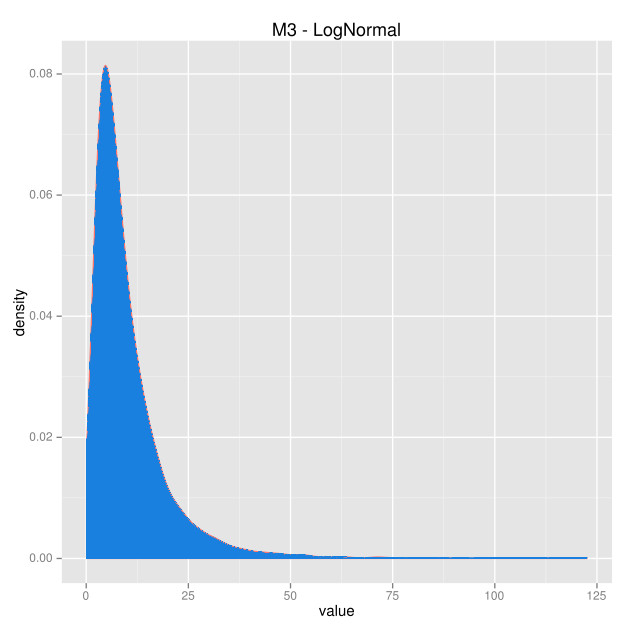
\includegraphics[height=0.5\textwidth]{./lognormal.jpg}
		\vfill
	
\end{center}	
\begin{center}
\tiny Parameters: mu (U(0.1,4)) sd (U(0.1,3))
\end{center}

\end{frame}

\begin{frame}{M4: Pareto distribution}
\begin{itemize}
\item 80\% of the market was dominated by 20\% of the producers
\item Common structure in current markets
\end{itemize}
\begin{center}
		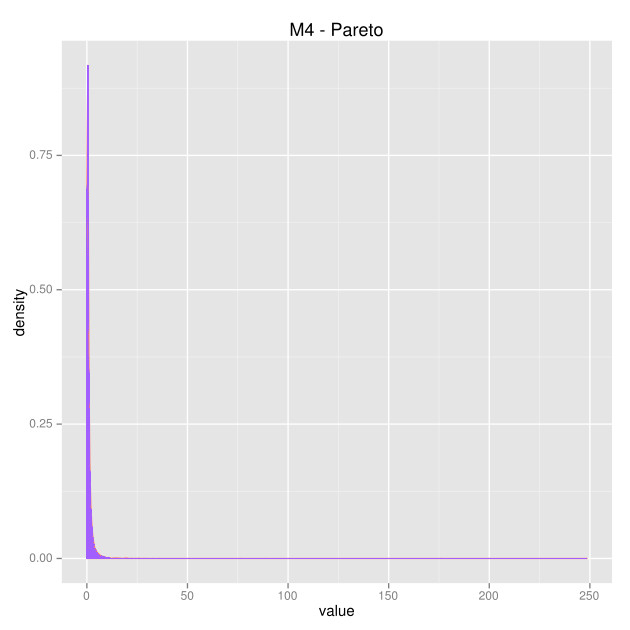
\includegraphics[height=0.5\textwidth]{./pareto.jpg}
		\vfill
	
\end{center}	
\begin{center}
\tiny Parameters: shape (U(0.1,10) xm (1)
\end{center}
\end{frame}


\begin{frame}{MCMc simulation}
 \begin{center}
 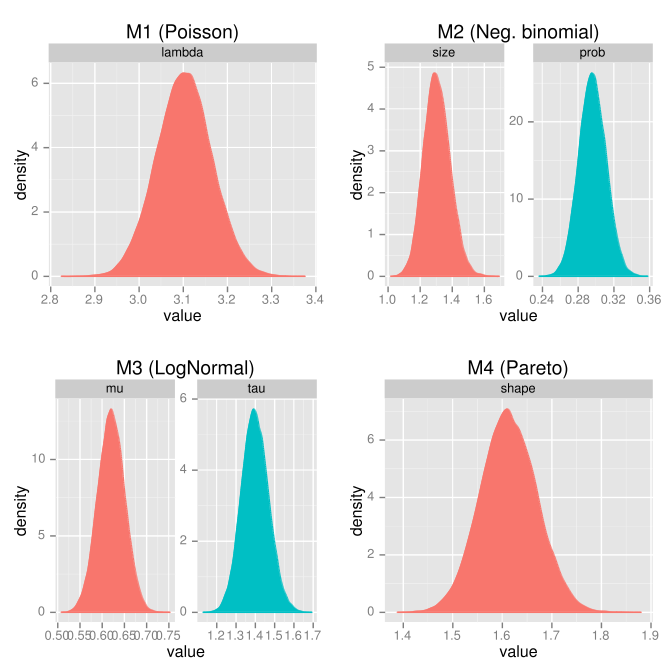
\includegraphics[height=0.6\textwidth]{./pareto2.png}
 \end{center}

\end{frame}

\section{Results and Discussion}

\begin{frame}{Deviance Information Criteria (DIC)}
\begin{itemize}
\item Smaller values 
\item M4 fits better to the evidence
\end{itemize}
\begin{center}
		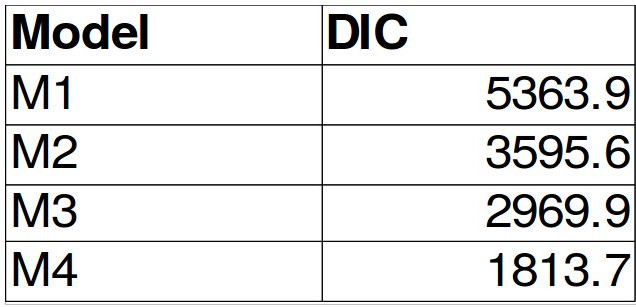
\includegraphics[height=0.3\textwidth]{./dictable.jpg}
		\vfill
	
\end{center}	
			
\end{frame}


\begin{frame}{Results}
\begin{itemize}
\item Our hypothesis fits to the models proposed
\item Last model is better to fit to the evidence
\item Large producers coexisted with the high presence of different small-size producers (different stamps)

\end{itemize}
\end{frame} 

\begin{frame}{Discussion}
\begin{itemize}
\item Results suggest the existence of a free market of olive oil production in the Roman Empire 
\item These results match the frequency distribution of current company sizes
\item Useful tool in contexts with high level of uncertainty such as Archaeology

\end{itemize}
\end{frame} 

\begin{frame}
\vspace{1cm}
\Huge Thank you for your attention!\\
                                    
\begin{center}
\normalsize                 
Mar\'ia Coto-Sarmiento\\
@mcotsar\\
maria.coto@bsc.es\\
Barcelona Supercomputing Center
\end{center}

\vspace{-.3cm}
\begin{center}
		
\includegraphics[height=0.12\textwidth]{./epnetlogo.jpg}
		
\includegraphics[height=0.1\textwidth]{./computing.jpg}
		 
\includegraphics[height=0.12\textwidth]{./ERC.png}
		\vfill
	
\end{center}		

\end{frame}

\begin{frame}

\begin{center}
 \centering
 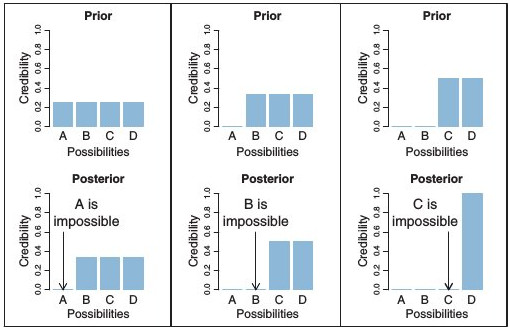
\includegraphics[height=0.5\textwidth]{./priorposterior.jpg}
 \end{center}


\end{frame} 

\end{document}